\documentclass[a4j, twocolumn, 8pt,pdflatex,jadriver=standard]{bxjsarticle}
\usepackage[dvipdfm]{graphicx}
\usepackage{amsmath,amssymb,bm}
\setlength{\headheight}{0mm}
\setlength{\headsep}{0mm}
\setlength{\footskip}{0mm}
%\setlength{\topmargin}{-30mm}
\setlength{\topmargin}{-14mm}
\setlength{\oddsidemargin}{-8mm}
\setlength{\evensidemargin}{-8mm}
%\setlength{\textheight}{290mm}
\setlength{\textheight}{274mm}
\setlength{\textwidth}{176mm}
%\renewcommand{\baselinestretch}{0.85}
%\renewcommand{\refname}{\large 参�??��献}

\renewcommand{\figurename}{図}
\renewcommand{\tablename}{表}
\def \figref  #1{\figurename\ref{#1}}
\def \tabref  #1{\tablename\ref{#1}}
\def \equref  #1{\ref{#1})}

\makeatletter
\renewcommand\maketitle{
  \ifnum \col@number=\@ne \@maketitle
  \else \twocolumn[
    \vspace{-16mm}
    \@maketitle
  ]
  \fi
 }
\makeatother

\pagestyle{empty}

\title{{\small $<$2016hogehoge[中間サーベイ論文$>$}\\
       {\Large 題名}\vspace{-4mm}}
\author{{\normalsize 機械学科03-123456機械太郎}\vspace{-4mm}}
%\date{\small 平成?8年 7月13日}
\date{\small \today}

\begin{document}
\maketitle \thispagestyle{empty}
\normalsize
\vspace{-8mm}


\section{はじめに}
\vspace{-3mm}

引用例~\cite{Brooks1991:Intelligence_Without_Reason}です
chukan.bib ファイルを作っておきbibtexを使って引用して日本語もOK~\cite{book:Pfeifer:知の創成}.

脚注\footnote{脚注はあんまり使ない}はこんな風に使
ちなみに句読点は「,」と「.」にそろえましょ
\section{目的}
\vspace{-3mm}
目的書きます
 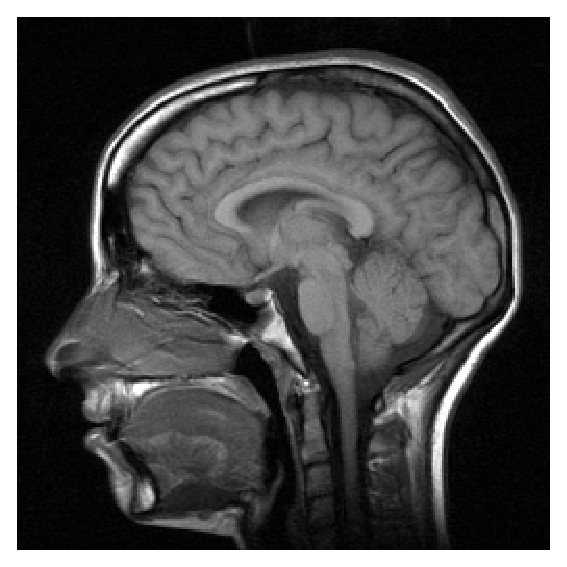
\includegraphics[width=7cm,clip]{./figure/map.eps}
\begin{figure}[htbp]
 \begin{center}
 \caption{MRI画像}
 \label{fig:mri}
 \end{center}
\end{figure}

\vspace{-9mm}
図はたとfigref{fig:mri}のように

abc $ \sum_{i=1}^N \sin \frac{\phi}{\pi}$
\begin{equation}
 \sum_{i=1}^N \sin \frac{\phi}{\pi}
\end{equation}

\vspace{-6mm}
\section{方法と計画}
\vspace{-3mm}
これからの方針を書きます�?
  \begin{table}[htbp]
    \begin{center}
      \caption{表の例}
      \label{table:table_example}
      \begin{tabular}{l|cccccc}
	\hline
	A & 1 & 2 & 3 & 4 & 5 & 6\\
	\hline
	B & a & b & c & d & e & f\\
	\hline
      \end{tabular}
    \end{center}
  \end{table}
表はたとえ\tabref{table:table_example}のように

\section{現在の進行状況}
こんなことてきました??
\section{今後の課題}
これからこんなことをやります
\small{
\begin{thebibliography}{9}
\vspace{-2mm}
\bibitem{Brooks}
 R.A.Brooks,``A Robust Layered Control System for a Mobile Robot'', IEEE J. Robotics And Automation, RA-2, pp.14-23, 1986.
\end{thebibliography}

%}
\small{
%\bibliographystyle{jplain}
\bibliographystyle{junsrt}
\bibliography{chukan}
}

\end{document}

